% Example quiz. Upload this file and triangle.png together.
% Text outside problems is metadata; no TeX installation is needed.
\documentclass{article}
\usepackage{amsmath,amssymb,graphicx}
\quiztitle{Mixed mathematics}
\quizdescription{Parity, congruences, geometry, counting, and probability.}
\quizsubject{Mixed topics}
\quizdifficulty{Olympiad}
\quiztime{20}
\begin{document}

\begin{problem}[points=2]
A sum of $2027$ odd integers is always:
\begin{choices}
\choice Even
\correctchoice Odd
\choice Divisible by $3$
\choice A prime number
\end{choices}
\begin{solution}
Each odd integer is congruent to $1$ modulo $2$, so the sum is congruent to $2027\equiv 1\pmod{2}$.
\end{solution}
\end{problem}

\begin{problem}[points=3]
Find the smallest positive integer $n$ for which
\[7n\equiv 1\pmod{10}.\]
\answer{3}
\begin{solution}
Since $7\cdot 3=21\equiv 1\pmod{10}$, and $n=1,2$ do not work, the answer is $3$.
\end{solution}
\end{problem}

\begin{problem}[points=2]
If $x+y=6$ and $xy=8$, what is $x^2+y^2$?
\begin{choices}
\choice $12$
\choice $16$
\correctchoice $20$
\choice $28$
\end{choices}
\begin{solution}
Use $x^2+y^2=(x+y)^2-2xy=36-16=20$.
\end{solution}
\end{problem}

\begin{problem}[points=3]
In triangle $ABC$, $\angle A=50^\circ$ and $\angle B=60^\circ$.
Find $\angle C$, in degrees. Enter the number only.
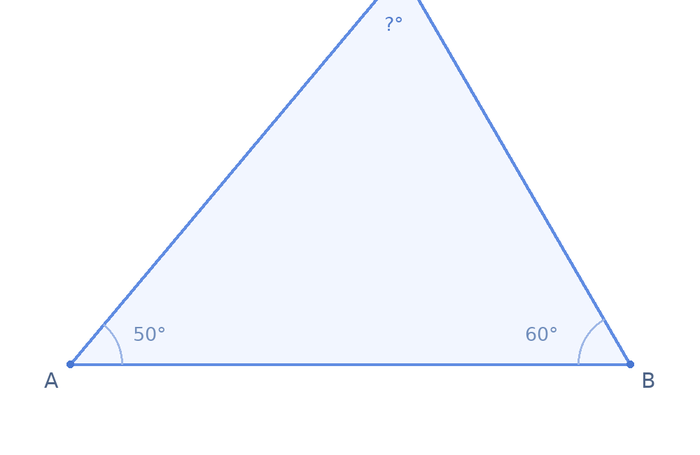
\includegraphics[width=0.8\linewidth]{triangle.png}
\answer{70}
\begin{solution}
The interior angles of a triangle sum to $180^\circ$, hence $\angle C=180^\circ-50^\circ-60^\circ=70^\circ$.
\end{solution}
\end{problem}

\begin{problem}[points=2]
How many subsets does a set with $4$ elements have, including the empty set?
\begin{choices}
\choice $8$
\choice $12$
\correctchoice $16$
\choice $24$
\end{choices}
\begin{solution}
Each element is either included or excluded. These independent choices give $2^4=16$ subsets.
\end{solution}
\end{problem}

\begin{problem}[points=3]
Find the sum
\[1+2+3+\cdots+100.\]
\answer{5050}
\begin{solution}
Pair the first and last terms to obtain $50\cdot101=5050$.
\end{solution}
\end{problem}

\begin{problem}[points=2]
Two diagonally opposite corners are removed from an $8\times8$ chessboard.
Can the remaining board be tiled with $1\times2$ dominoes?
\begin{choices}
\choice Yes, for every such pair of corners
\choice Yes, but only using vertical dominoes
\correctchoice No
\choice There is not enough information
\end{choices}
\begin{solution}
The removed squares have the same colour. Every domino covers one square of each colour, but the remaining board has unequal numbers of the two colours.
\end{solution}
\end{problem}

\begin{problem}[points=3,tolerance=0.000001]
Two fair six-sided dice are rolled. What is the probability that their sum is $7$?
You may enter a fraction.
\answer{1/6}
\accepted{\frac{1}{6}}
\begin{solution}
There are $6$ favourable ordered outcomes among $36$ equally likely outcomes. The probability is $6/36=1/6$.
\end{solution}
\end{problem}
\end{document}
